\documentclass[12pt]{article}
\usepackage{amsmath}
\usepackage{graphicx}
\usepackage{hyperref}
\usepackage{listings}
\usepackage{color}
\usepackage{pythonhighlight}

\title{Operating System Course Report - First Half of the Semester}
\author{B class}
\date{\today}

\begin{document}

\maketitle
\newpage

\tableofcontents
\newpage

\section{Introduction}
This report summarizes the topics covered during the first half of the Operating System course. It includes theoretical concepts, practical implementations, and assignments. The course focuses on the fundamentals of operating systems, including system architecture, process management, CPU scheduling, and deadlock handling.

\section{Course Overview}
\subsection{Objectives}
The main objectives of this course are:
\begin{itemize}
    \item To understand the basic components and architecture of a computer system.
    \item To learn process management, scheduling, and inter-process communication.
    \item To explore file systems, input/output management, and virtualization.
    \item To study the prevention and handling of deadlocks in operating systems.
\end{itemize}

\subsection{Course Structure}
The course is divided into two halves. This report focuses on the first half, which covers:
\begin{itemize}
    \item Basic Concepts and Components of Computer Systems
    \item System Performance and Metrics
    \item System Architecture of Computer Systems
    \item Process Description and Control
    \item Scheduling Algorithms
    \item Process Creation and Termination
    \item Introduction to Threads
    \item File Systems
    \item Input and Output Management
    \item Deadlock Introduction and Prevention
    \item User Interface Management
    \item Virtualization in Operating Systems
\end{itemize}

\section{Topics Covered}

\subsection{Basic Concepts and Components of Computer Systems}
This section explains the fundamental components that make up a computer system, including the CPU, memory, storage, and input/output devices.

\subsection{System Performance and Metrics}
This section introduces various system performance metrics used to measure the efficiency of a computer system, including throughput, response time, and utilization.

\subsection{System Architecture of Computer Systems}
Describes the architecture of modern computer systems, focusing on the interaction between hardware and the operating system.

\subsection{Process Description and Control}
\subsubsection{Definition of Process}
Proses adalah program yang sedang dieksekusi, yang terdiri dari instruksi yang berjalan pada CPU, serta informasi yang diperlukan untuk menjalankan program tersebut. Setiap proses memiliki siklus hidup yang melibatkan berbagai keadaan (states) dan transisi antar keadaan tersebut.

\subsubsection{Process states and state transitions}
Keadaan proses merujuk pada status atau fase yang dilalui oleh suatu proses selama siklus hidupnya. Setiap proses dapat berada dalam salah satu dari beberapa keadaan yang berbeda, dan transisi antar keadaan ini diatur oleh sistem operasi untuk memastikan manajemen proses yang efisien. Berikut adalah beberapa keadaan utama yang biasanya diidentifikasi dalam sistem operasi:

\begin{figure}[h]
        \centering
        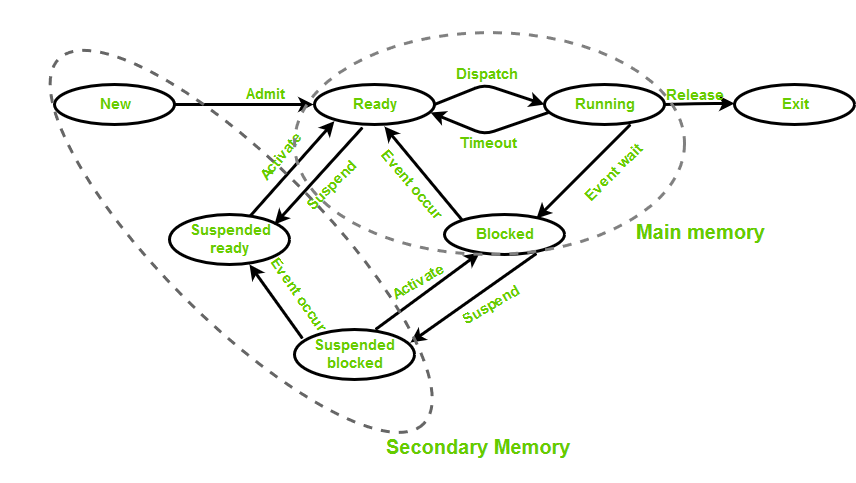
\includegraphics[width=0.6\textwidth]{asset/gambar_keadaan_proses.png}
        \caption{gambar keadaan dalam proses}
\end{figure}

\begin{itemize}
    \item \textbf{New (Baru)}: Proses baru saja dibuat. Pada keadaan ini, proses sedang dalam tahap inisialisasi, di mana sistem operasi mengalokasikan sumber daya yang diperlukan seperti memori dan ID proses.
    \item \textbf{Ready (Siap)}: Proses telah siap untuk dieksekusi tetapi belum mendapatkan akses ke CPU. Proses ini menunggu dalam antrean ready hingga sistem operasi memilihnya untuk dieksekusi. Proses dalam keadaan ini dapat dipindahkan kembali ke antrean jika CPU sedang sibuk.
    \item \textbf{Running (Berjalan)}: Proses sedang dieksekusi oleh CPU. Pada keadaan ini, instruksi proses sedang dijalankan. CPU memberikan waktu eksekusi untuk proses dalam keadaan ini.
    \item \textbf{Waiting (Menunggu)}: Proses tidak dapat melanjutkan eksekusi hingga suatu event tertentu terjadi seperti menyelesaikan operasi I/O. Ketika menunggu, proses tidak dapat menggunakan CPU dan akan pindah ke antrean waiting.
    \item \textbf{Terminated (Selesai)}: Proses telah selesai menjalankan semua instruksinya. Semua sumber daya yang dialokasikan untuk proses tersebut dibebaskan, dan sistem operasi memperbarui status proses menjadi terminated.
\end{itemize}

Transisi antara keadaan proses ini adalah bagian penting dari manajemen proses. Berikut adalah beberapa transisi umum:
\begin{itemize}
    \item \textbf{New → Ready}: Ketika proses berhasil dibuat dan siap untuk dijadwalkan.
    \item \textbf{Ready → Running}: Ketika CPU memilih proses dari antrean ready untuk dieksekusi.
    \item \textbf{Running → Waiting}: Ketika proses membutuhkan I/O atau menunggu event tertentu (misalnya menyelesaikan pembacaan dari disk).
    \item \textbf{Running → Ready}: Ketika proses di-preempt karena waktu eksekusi habis atau ada proses dengan prioritas lebih tinggi yang memerlukan CPU.
    \item \textbf{Waiting → Ready}: Ketika event yang ditunggu oleh proses selesai, proses tersebut kembali ke antrean ready.
    \item \textbf{Running → Terminated}: Ketika proses selesai menjalankan semua instruksinya.
\end{itemize}

\subsubsection{Process Control Block (PCB)}
\subsubsection{Context Switching}
\subsubsection{Process Management By Operating Systems}

\subsection{Scheduling Algorithms}
This section covers:
\begin{itemize}
    \item First-Come, First-Served (FCFS)
    \item Shortest Job Next (SJN)
    \item Round Robin (RR)
\end{itemize}
It explains how these algorithms are used to allocate CPU time to processes.

\subsection{Process Creation and Termination}
Details how processes are created and terminated by the operating system, including:
\begin{itemize}
    \item Process spawning
    \item Process termination conditions
\end{itemize}

\subsection{Introduction to Threads}
This section introduces the concept of threads and their relation to processes, covering:
\begin{itemize}
    \item Single-threaded vs. multi-threaded processes
    \item Benefits of multithreading
\end{itemize}

\begin{figure}[h]
    \centering
    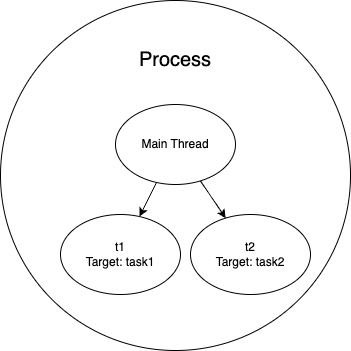
\includegraphics[width=0.5\textwidth]{asset/example.png}  % Sesuaikan nama file dan ukurannya
    \caption{Ini adalah gambar contoh dari multithreading.}
    \label{fig:contoh_gambar}
\end{figure}

Seperti yang terlihat pada Gambar \ref{fig:contoh_gambar}, inilah cara menambahkan gambar dengan keterangan.

\subsection{File Systems}
File systems provide a way for the operating system to store, retrieve, and manage data. This section explains:
\begin{itemize}
    \item File system structure
    \item File access methods
    \item Directory management
\end{itemize}

\subsection{Input and Output Management}
Input and output management is key for handling the interaction between the system and external devices. This section includes:
\begin{itemize}
    \item Device drivers
    \item I/O scheduling
\end{itemize}

\subsection{Deadlock Introduction and Prevention}
Explores the concept of deadlocks and methods for preventing them:
\begin{itemize}
    \item Deadlock conditions
    \item Deadlock prevention techniques
\end{itemize}

\subsection{User Interface Management}
This section discusses the role of the operating system in managing the user interface. Topics covered include:
\begin{itemize}
    \item Graphical User Interface (GUI)
    \item Command-Line Interface (CLI)
    \item Interaction between the user and the operating system
\end{itemize}

\subsection{Virtualization in Operating Systems}
Virtualization allows multiple operating systems to run concurrently on a single physical machine. This section explores:
\begin{itemize}
    \item Concept of virtualization
    \item Hypervisors and their types
    \item Benefits of virtualization in modern computing
\end{itemize}

\section{Assignments and Practical Work}
\subsection{Assignment 1: Process Scheduling}
Students were tasked with implementing various process scheduling algorithms (e.g., FCFS, SJN, and RR) and comparing their performance under different conditions.
\subsubsection{Group 1}
\begin{python}
    class Process:
    def __init__(self, pid, arrival_time, burst_time):
        self.pid = pid
        self.arrival_time = arrival_time
        self.burst_time = burst_time
        self.completion_time = 0
        self.turnaround_time = 0
        self.waiting_time = 0
\end{python}

\begin{table}[htbp] % Optional: For floating position
    \centering
    \begin{tabular}{|c|c|c|} % Defines number of columns and alignment (c = center, l = left, r = right). '|' creates vertical lines.
    \hline
    Header 1 & Header 2 & Header 3 \\ % Column headers
    \hline
    Row 1, Column 1 & Row 1, Column 2 & Row 1, Column 3 \\ % First row of data
    \hline
    Row 2, Column 1 & Row 2, Column 2 & Row 2, Column 3 \\ % Second row of data
    \hline
    \end{tabular}
    \caption{Your table caption} % Optional: For adding a caption
    \label{tab:your_label} % Optional: For cross-referencing the table
\end{table}

\subsection{Assignment 2: Deadlock Handling}
\subsubsection{Pengertian Deadlock}
Deadlock adalah kondisi di mana dua atau lebih proses saling menunggu sumber daya yang sedang dipegang oleh proses lain, sehingga tidak ada satu pun proses yang dapat melanjutkan eksekusinya. Deadlock dapat terjadi jika keempat kondisi berikut terpenuhi secara bersamaan:
\begin{enumerate}
    \item \textbf{Mutual Exclusion (Eksklusi Mutual)}: Sumber daya hanya dapat digunakan oleh satu proses pada satu waktu.
    \item \textbf{Hold and Wait (Menahan dan Menunggu)}: Proses yang sudah memiliki sumber daya dapat meminta sumber daya tambahan tanpa melepaskan sumber daya yang sedang dipegangnya.
    \item \textbf{No Preemption (Tanpa Preempesi)}: Sumber daya yang dimiliki oleh suatu proses tidak dapat diambil secara paksa.
    \item \textbf{Circular Wait (Menunggu Melingkar)}: Proses-proses membentuk siklus di mana setiap proses menunggu sumber daya yang sedang dipegang oleh proses berikutnya dalam siklus tersebut.
\end{enumerate}

\subsubsection{Metode Pencegahan Deadlock}
Untuk mengatasi deadlock, terdapat beberapa metode yang dapat digunakan:
\begin{enumerate}
    \item \textbf{Avoidance (Penghindaran)}: Menggunakan algoritma seperti Algoritma Bankir untuk menghindari sistem memasuki kondisi deadlock.
    \item \textbf{Prevention (Pencegahan)}: Mengubah salah satu dari empat kondisi deadlock agar deadlock tidak terjadi.
    \item \textbf{Detection and Recovery (Deteksi dan Pemulihan)}: Membiarkan deadlock terjadi, kemudian mendeteksi dan mengambil tindakan pemulihan seperti menghentikan salah satu proses.
\end{enumerate}

\subsubsection{Contoh Kasus Deadlock}
Misalkan terdapat tiga proses yang bersaing untuk mendapatkan tiga jenis sumber daya: A, B, dan C. Setiap jenis sumber daya memiliki 10 unit. Proses-proses tersebut adalah sebagai berikut:

\begin{itemize}
    \item P1 memiliki 3 unit A, 2 unit B, dan 2 unit C, serta membutuhkan tambahan 1 unit A, 1 unit B, dan 3 unit C.
    \item P2 memiliki 2 unit A, 3 unit B, dan 3 unit C, serta membutuhkan tambahan 2 unit A, 1 unit B, dan 2 unit C.
    \item P3 memiliki 1 unit A, 2 unit B, dan 2 unit C, serta membutuhkan tambahan 4 unit A, 2 unit B, dan 2 unit C.
\end{itemize}

Apakah sistem ini dalam kondisi deadlock? Jika iya, bagaimana cara menghindarinya menggunakan Algoritma Bankir?

\subsubsection{Implementasi Algoritma Bankir}
Berikut adalah contoh kode Python untuk mensimulasikan Algoritma Bankir:

\begin{python}
    
    # Algoritma Bankir dalam Python
    
    # Jumlah proses dan sumber daya
    P = 3  # Jumlah proses
    R = 3  # Jumlah jenis sumber daya (A, B, C)
    
    # Sumber daya yang tersedia
    available = [3, 3, 2]  # A = 3, B = 3, C = 2 (Sumber daya yang tersedia)
    
    # Permintaan maksimum dari masing-masing proses
    max_demand = [
        [7, 5, 3],  # Permintaan maksimum P1 untuk A, B, C
        [3, 2, 2],  # Permintaan maksimum P2
        [9, 0, 2]   # Permintaan maksimum P3
    ]
    
    # Sumber daya yang saat ini dialokasikan untuk masing-masing proses
    allocated = [
        [3, 2, 2],  # Sumber daya yang dialokasikan untuk P1
        [2, 0, 0],  # Sumber daya yang dialokasikan untuk P2
        [3, 0, 2]   # Sumber daya yang dialokasikan untuk P3
    ]
    
    # Menghitung matriks kebutuhan (max_demand - allocated)
    def calculate_need(max_demand, allocated):
        need = []
        for i in range(P):
            need.append([max_demand[i][j] - allocated[i][j] for j in range(R)])
        return need
    
    # Fungsi untuk memeriksa apakah sistem dalam kondisi aman
    def is_safe(available, max_demand, allocated):
        need = calculate_need(max_demand, allocated)
        work = available[:]
        finish = [False] * P
        safe_sequence = []
    
        while len(safe_sequence) < P:
            found_process = False
            for i in range(P):
                if not finish[i]:
                    if all(need[i][j] <= work[j] for j in range(R)):
                        # Jika proses dapat diselesaikan
                        for j in range(R):
                            work[j] += allocated[i][j]
                        finish[i] = True
                        safe_sequence.append(i)
                        found_process = True
    
            if not found_process:
                break
    
        if len(safe_sequence) == P:
            print(f"Sistem berada dalam keadaan aman.\nUrutan aman: {safe_sequence}")
            return True
        else:
            print("Sistem berada dalam kondisi deadlock.")
            return False
    
    # Memeriksa apakah sistem dalam keadaan aman
    is_safe(available, max_demand, allocated)
\end{python}

\subsubsection{Penjelasan Kode}
\begin{itemize}
    \item \textbf{available}: Jumlah sumber daya yang tersedia untuk masing-masing jenis (A, B, dan C).
    \item \textbf{max\_demand}: Matriks yang menunjukkan permintaan maksimum sumber daya untuk setiap proses.
    \item \textbf{allocated}: Matriks yang menunjukkan jumlah sumber daya yang telah dialokasikan untuk masing-masing proses.
    \item \textbf{calculate\_need}: Fungsi untuk menghitung sumber daya yang masih dibutuhkan oleh setiap proses.
    \item \textbf{is\_safe}: Fungsi utama yang menentukan apakah sistem berada dalam keadaan aman (safe state) atau dalam kondisi deadlock, menggunakan Algoritma Bankir.
\end{itemize}

Jika sistem berada dalam kondisi aman, program akan menampilkan pesan:
\begin{python}
    
Sistem berada dalam keadaan aman.
Urutan aman: [0, 2, 1]
\end{python}

Jika sistem berada dalam kondisi deadlock, program akan menampilkan pesan:
\begin{python}
    System is in a deadlock.
\end{python}


\subsection{Assignment 3: Multithreading and Amdahl's Law}
This assignment involved designing a multithreading scenario to solve a computationally intensive problem. Students then applied **Amdahl's Law** to calculate the theoretical speedup of the program as the number of threads increased.

\subsection{Assignment 4: Simple Command-Line Interface (CLI) for User Interface Management}
Pada tugas ini, diminta untuk membuat Command-Line Interface (CLI) sederhana yang digunakan untuk manajemen antarmuka pengguna. Tujuan utama dari CLI ini adalah untuk memberikan kontrol dasar bagi pengguna dalam mengelola file, proses, serta memantau status sistem melalui serangkaian perintah yang mudah digunakan. Dengan CLI ini, pengguna akan dapat melakukan operasi-operasi seperti pembuatan, penghapusan, dan penampilan file, serta manajemen proses yang berjalan di sistem operasi.

\subsubsection{Tujuan}
Untuk membuat sebuah CLI sederhana yang dapat menangani pengelolaan file, manajemen proses, dan pelaporan status sistem. Fitur utama yang harus disediakan meliputi:

\begin{itemize}
    \item Manipulasi file: membuat, menampilkan, dan menghapus file.
    \item Manajemen proses: menampilkan proses yang berjalan dan menghentikan proses berdasarkan PID (Process ID).
    \item Pelaporan status sistem: menampilkan informasi tentang memori dan ruang penyimpanan yang digunakan.
\end{itemize}


\subsubsection{\textbf{Fitur CLI}}

\textbf{CLI} harus mampu menerima perintah pengguna dan menjalankan fungsi yang sesuai, seperti:

\begin{itemize}
    \item Membuat file baru.
    \item Menampilkan daftar file dalam direktori saat ini.
    \item Menghapus file yang ada.
    \item Menampilkan daftar proses yang sedang berjalan.
    \item Menghentikan proses berdasarkan \textbf{PID}.
    \item Menampilkan status memori dan ruang penyimpanan sistem.
\end{itemize}

\subsubsection{Penjelasan Fitur}

Berikut adalah penjelasan dari setiap fitur CLI yang harus dibuat:

\paragraph{a. \textbf{Manipulasi File}}

\begin{enumerate}
    \item \textbf{Membuat File}: Mengizinkan pengguna membuat file teks dengan isi yang diinginkan.
    \item \textbf{Menampilkan Daftar File}: Menampilkan semua file yang ada dalam direktori saat ini.
    \item \textbf{Menghapus File}: Menghapus file berdasarkan nama yang diberikan pengguna.
\end{enumerate}

\paragraph{b. \textbf{Manajemen Proses}}

\begin{enumerate}
    \item \textbf{Menampilkan Daftar Proses}: Menampilkan semua proses yang sedang berjalan di sistem, beserta PID dan nama proses.
    \item \textbf{Menghentikan Proses}: Menghentikan proses yang dipilih pengguna berdasarkan \textbf{PID} yang diberikan.
\end{enumerate}

\paragraph{c. \textbf{Pelaporan Status Sistem}}

\begin{enumerate}
    \item \textbf{Status Memori}: Menampilkan informasi tentang penggunaan memori sistem (seberapa besar memori yang digunakan).
    \item \textbf{Ruang Penyimpanan}: Menampilkan status penggunaan ruang penyimpanan pada sistem.
\end{enumerate}


\subsubsection{\textbf{Contoh Soal}}

\textbf{Soal:} Buatlah sebuah program Python yang berfungsi sebagai CLI sederhana untuk melakukan:

\begin{enumerate}
    \item Membuat file teks baru dengan nama dan isi yang diinginkan.
    \item Menampilkan daftar file dalam direktori saat ini.
    \item Menghapus file yang dipilih pengguna.
    \item Menampilkan proses yang sedang berjalan di sistem.
    \item Menghentikan proses berdasarkan \textbf{PID}.
    \item Menampilkan informasi status sistem, seperti penggunaan memori dan ruang penyimpanan.
\end{enumerate}

 
\subsubsection{\textbf{Contoh Kode Python}}

Berikut adalah implementasi Python untuk menjawab soal tersebut

\begin{python}
    
    import os
    import psutil  # Library untuk mengelola proses dan status sistem
    
    # Fungsi untuk membuat file
    def create_file():
        filename = input("Masukkan nama file: ")
        content = input("Masukkan isi file: ")
        with open(filename, "w") as file:
            file.write(content)
        print(f"File '{filename}' berhasil dibuat.")
    
    # Fungsi untuk menampilkan daftar file
    def list_files():
        files = os.listdir()
        print("Daftar file di direktori saat ini:")
        for file in files:
            print(f"- {file}")
    
    # Fungsi untuk menghapus file
    def delete_file():
        filename = input("Masukkan nama file yang ingin dihapus: ")
        if os.path.exists(filename):
            os.remove(filename)
            print(f"File '{filename}' berhasil dihapus.")
        else:
            print("File tidak ditemukan.")
    
    # Fungsi untuk menampilkan daftar proses
    def list_processes():
        print("Proses yang sedang berjalan:")
        for proc in psutil.process_iter(['pid', 'name']):
            print(f"PID: {proc.info['pid']}, Nama: {proc.info['name']}")
    
    # Fungsi untuk menghentikan proses berdasarkan PID
    def kill_process():
        pid = int(input("Masukkan PID proses yang ingin dihentikan: "))
        try:
            p = psutil.Process(pid)
            p.terminate()
            print(f"Proses dengan PID {pid} berhasil dihentikan.")
        except psutil.NoSuchProcess:
            print("Proses tidak ditemukan.")
    
    # Fungsi untuk menampilkan status sistem
    def system_status():
        memory = psutil.virtual_memory()
        storage = psutil.disk_usage('/')
        print(f"Status Memori: {memory.percent}% digunakan")
        print(f"Ruang Penyimpanan: {storage.percent}% digunakan")
    
    # Fungsi utama CLI
    def cli():
        while True:
            print("\n=== CLI Sederhana ===")
            print("1. Buat file")
            print("2. Tampilkan daftar file")
            print("3. Hapus file")
            print("4. Tampilkan daftar proses")
            print("5. Hentikan proses")
            print("6. Tampilkan status sistem")
            print("7. Keluar")
            choice = input("Pilih opsi (1-7): ")
    
            if choice == '1':
                create_file()
            elif choice == '2':
                list_files()
            elif choice == '3':
                delete_file()
            elif choice == '4':
                list_processes()
            elif choice == '5':
                kill_process()
            elif choice == '6':
                system_status()
            elif choice == '7':
                print("Keluar dari CLI.")
                break
            else:
                print("Pilihan tidak valid, silakan coba lagi.")
    
    # Memulai CLI
    cli()
\end{python}


\subsubsection{\textbf{Penjelasan Kode}}

\begin{itemize}
    \item \textbf{create\_file}: Fungsi ini membuat file baru berdasarkan nama dan isi yang dimasukkan oleh pengguna.
    \item \textbf{list\_files}: Menampilkan semua file di direktori saat ini.
    \item \textbf{delete\_file}: Menghapus file yang dipilih pengguna.
    \item \textbf{list\_processes}: Menampilkan daftar proses yang berjalan di sistem.
    \item \textbf{kill\_process}: Menghentikan proses yang dipilih berdasarkan \textbf{PID}.
    \item \textbf{system\_status}: Menampilkan informasi penggunaan memori dan ruang penyimpanan sistem.
\end{itemize}

\subsubsection{Kesimpulan}

Program ini memungkinkan  untuk mengelola file, mengawasi proses, dan memantau status sistem melalui antarmuka baris perintah (CLI). Ini membantu memahami dasar-dasar manajemen file dan proses dalam lingkungan berbasis teks.

 
\subsection{Assignment 5: File System Access}
In this assignment, students implemented file system access routines, including:
\begin{itemize}
    \item File creation and deletion
    \item Reading from and writing to files
    \item Navigating directories and managing file permissions
\end{itemize}

\section{Conclusion}
The first half of the course introduced core operating system concepts, including process management, scheduling, multithreading, and file system access. These topics provided a foundation for more advanced topics to be covered in the second half of the course.

%\section*{Daftar Pustaka}

\begin{thebibliography}{}

\bibitem{}
GeeksforGeeks. (n.d.). \textit{Process states in operating system}. Diakses pada 30 September 2024, dari \url{https://www.geeksforgeeks.org/process-states-in-operating-system/}

\bibitem{}
Tutorialspoint. (n.d.). \textit{Operating system - Process control block}. Diakses pada 30 September 2024, dari \url{https://www.tutorialspoint.com/operating_system/os_process_control_block.htm}

\bibitem{}
Wikipedia contributors. (n.d.). Context switch. Dalam \textit{Wikipedia, The Free Encyclopedia}. Diakses pada 30 September 2024, dari \url{https://en.wikipedia.org/wiki/Context_switch}

\end{thebibliography}

\end{document}